% Chapter Template

\chapter{Implementation} % Main chapter title

\label{introduction} % Change X to a consecutive number; for referencing this chapter elsewhere, use \ref{ChapterX}

\lhead{Chapter 5. \emph{Implementation}} % Change X to a consecutive number; this is for the header on each page - perhaps a shortened title

%----------------------------------------------------------------------------------------
%	SECTION 1
%----------------------------------------------------------------------------------------

Sed ullamcorper quam eu nisl interdum at interdum enim egestas. Aliquam placerat justo sed lectus lobortis ut porta nisl porttitor. Vestibulum mi dolor, lacinia molestie gravida at, tempus vitae ligula. Donec eget quam sapien, in viverra eros. Donec pellentesque justo a massa fringilla non vestibulum metus vestibulum. Vestibulum in orci quis felis tempor lacinia. Vivamus ornare ultrices facilisis. Ut hendrerit volutpat vulputate. Morbi condimentum venenatis augue, id porta ipsum vulputate in. Curabitur luctus tempus justo. Vestibulum risus lectus, adipiscing nec condimentum quis, condimentum nec nisl. Aliquam dictum sagittis velit sed iaculis. Morbi tristique augue sit amet nulla pulvinar id facilisis ligula mollis. Nam elit libero, tincidunt ut aliquam at, molestie in quam. Aenean rhoncus vehicula hendrerit.

\section{Case 1: Gas dispersion in a simplified urban area}
The problem investigated in this work is gas dispersion of neutral gas in a velocity field through four cubic blocks.
Similar simulations have been done in CDP and Fluent which are compared to data from a wind-tunnel experiment performed by ALAN.
\begin{itemize}
	\item Description of problem and domain
	\item mesh and fluent/CDP mesh
\end{itemize}

\section{Case 2: Drag and lift on a cylinder}
Descrition of problem\ldots
Descrition of implementation approach in Nek\ldots

\section{Advances in the mesh-generation routine}
The routine xyzarc:

The gordon hall algorithm was already implemented as a function in Nek, with the gll-points,plynomial degree and some initial 
coordinates to the element. The algorithm creates a distribution of the internal gll-points in each element. 
If the element consists of linear edges the only necessary input are the vertices, but by specifying the points on edges and faces
the algorithm creates a logical distribution of the internal GLL-points to a deformed element. 

The curved edge is specified in the .rea file and the routine genxyz() processes the input of each edge. 
By specifying the radius and the circle center genxyz calls the routine xyzarc() which performs the following algorithm;

    $a,b$ will be the two endnodes of the edge 
    $c$ will be the midnode, $s$ will be the arc length, $\theta$ will be the full angle of the circle sector, $cc$ is the center coordinates.
    $g$ will be the vector containing the GLL-points in $[-1,1]$. $r$ will be the radius.

	%/* Pseudo code */
%define interpolation algorithm 
%\textbf{\textbf{for}} each timestep \emph{T}
  %Read inflow
  %\textbf{for} each node \emph{N} and velocity component \emph{V} on inflow boundary 
    %\emph{V}(\emph{N}) = doInterpolation(N)
  %\textbf{endfor}
  %solve
%\textbf{endfor}
\begingroup
\fontsize{12pt}{14pt}
\begin{lstlisting}[escapechar=|]
 l = a-b                       # vector between the corner nodes
 c = (a+b)/2                   # midpoint location
 h = c-cc                      # height of the framed triangle
 |$\theta$| = arctan(abs(l)/2abs(h))    # half the angle of the circle sector
 s = r*|$\theta$|                       # arclength
 g' = g*|$\theta$|                      # angles to the gll-points on the circle-sector
 #---------- Finding the intersecting points ----------#
 #---- x on the line l, and extend x-cc to the arc ----#
 |\textbf{for}| k in range(lx1):          # For the number of nodes in one direction
    |$\alpha$| = h*tan(g'[k])           # Offset from the midpoint on l
    x = c-|$\alpha$|*l/abs(l)           # Actual coordinate on l
    m = x-cc                   # hypothenus of the imposed triangle
    edge(k) = cc+r*m/abs(m)    # final coordinate on the arc
\end{lstlisting}
\endgroup
These lines creates the wanted egde curved as a circle sector corresponding to the radius and circle center given.
The remaining operation is to call the gordon hall algorithm and create the internal GLL-points defined by the edges 
provided. The figure~\ref{fig:curvature} illustrates the geometry on which the algorithm is performed.
Notice that the algorithm assumes that the center is somewhere on the plane defined as all the 
points with equal distance to both $a$ and $b$.


\begin{figure}[h]
    \centering
    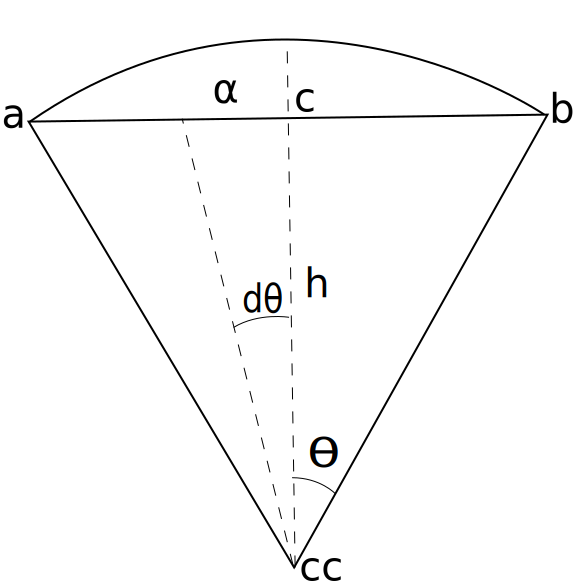
\includegraphics[width = 0.5\textwidth]{Figures/curvature.pdf}
    \caption{A sketch of the curved edge and the variables necessary to calculate the projection}
    \label{fig:curvature}
\end{figure}


\begin{itemize}
	\item initial script
	\item changes and modifications
	\item performance testing
	\item pitfalls
\end{itemize}


